\chapter{Umgang mit HDFS und MapReduce}
Zur Installation von Hadoop kann man die offizielle Distribution\footnote{https://hadoop.apache.org/releases.html} benutzen und komplett selbst konfigurieren. Dabei besteht die Möglichkeit, Hadoop in drei verschiedenen Modi zu betreiben: \textbf{Single Node}, \textbf{Pseudo-distributed} und \textbf{Fully-distributed}. Erstere beide sind zum Testen und Entwickeln, letztere für den tatsächlichen Einsatz im Cluster gedacht\cite[vgl.][Kap. 3.4]{freiknecht_big_2018}.
Weiterhin haben diverse kommerzielle Anbieter wie Cloudera\footnote{https://de.cloudera.com/} eigene Hadoop Distributionen entwickelt, die sie in Form von vorkonfigurierten VM- oder Docker-Images teilweise kostenlos zur Verfügung stellen. Cloudera zum Beispiel ergänzt diese Distributionen aber mittlerweile durch Cloudlösungen\footnote{https://de.cloudera.com/products/cloudera-data-platform.html}.   
Cloudanbieter wie Amazon, Google und Microsoft bieten fertig konfigurierte und voll verwaltete Cluster auf ihren jeweiligen Cloudplattformen an (Amazon EMR\footnote{https://aws.amazon.com/emr/features/hadoop/}, Google Dataproc\footnote{https://cloud.google.com/dataproc} und Azure HDInsight\footnote{https://azure.microsoft.com/en-us/products/hdinsight/\#overview}). 

\section{Single Node Setup}
Hadoop bietet unzählige Einstellungsmöglichkeiten während der Installation und sie alle zu behandeln würde den Rahmen dieser Arbeit sprengen. Daher wird in diesem Abschnitt ein VirtualBox Image von Cloudera (die Hortonworks Data Platform (HDP) Sandbox)\footnote{Download: https://www.cloudera.com/downloads/hortonworks-sandbox/hdp.html} genutzt. Dieses kann auf dem eigenen Rechner oder auf einem Remote-Host gestartet werden\footnote{Installation: https://www.cloudera.com/tutorials/sandbox-deployment-and-install-guide.html} und bietet Zugriff auf eine voll konfigurierte Installation von Hadoop im Single Node Modus. Zusätzlich sind noch ergänzende Komponenten aus dem Hadoop Ecosystem installiert, auf die in späteren Kapiteln eingegangen wird.

\section{Hadoop und Ambari in der HDP Sandbox VM}
Im Single Node Modus laufen alle Hadoop-Prozesse auf \textit{einem} Host(sprich Rechner). Dieser Modus ist für die Entwicklung und zum Testen von Hadoop gedacht, da es keinen praktischen Nutzen bringt, ein Framework zur verteilten Datenverarbeitung ohne die entsprechende Verteilung über einen Cluster zu betreiben. Auch wenn in dieser VM nur ein Cluster bestehend aus einem Node aufgesetzt wurde, steht das Cluster-Verwaltungs-Tool \textbf{Apache Ambari}\footnote{https://ambari.apache.org/} zur Verfügung. Normalerweise ist das Aufsetzen eines Hadoop Clusters mit dem Bearbeiten vieler XML-Konfigurationsdateien und der Ausführung von Start-Bash-Skripten auf allen Nodes verbunden. Auf diese Weise bestimmt man, welcher Node der NameNode des HDFS werden soll, welche Nodes DataNodes werden, wo der ResourceManager von YARN läuft und so weiter. Ambari bietet einem für all das (und noch viel mehr) eine übersichtliche Weboberfläche. Diese erreicht man nach Starten der HDP Sandbox unter \verb|http://localhost:8080|. Die Rechte und Anwendungsszenarien der verschiedenen Nutzeraccounts, eine Anleitung zum (Zurück)setzen des Admin-Passworts und weitere Schrite nach der Installation findet man auf Clouderas Hilfeseite zur Sandbox\footnote{https://www.cloudera.com/tutorials/learning-the-ropes-of-the-hdp-sandbox.html}. Loggt man sich als 'admin' zeitnah nach dem Start der VM in das das Ambari Dashboard ein, kann man im Header des Dashboards auf das Zahnrad klicken und den Prozess in Arbeit sehen, der die Dienste aller Hadoop Komponenten startet (siehe Abb. \ref{fig:cluster startup}). 

\begin{figure}[ht]
    \centering
    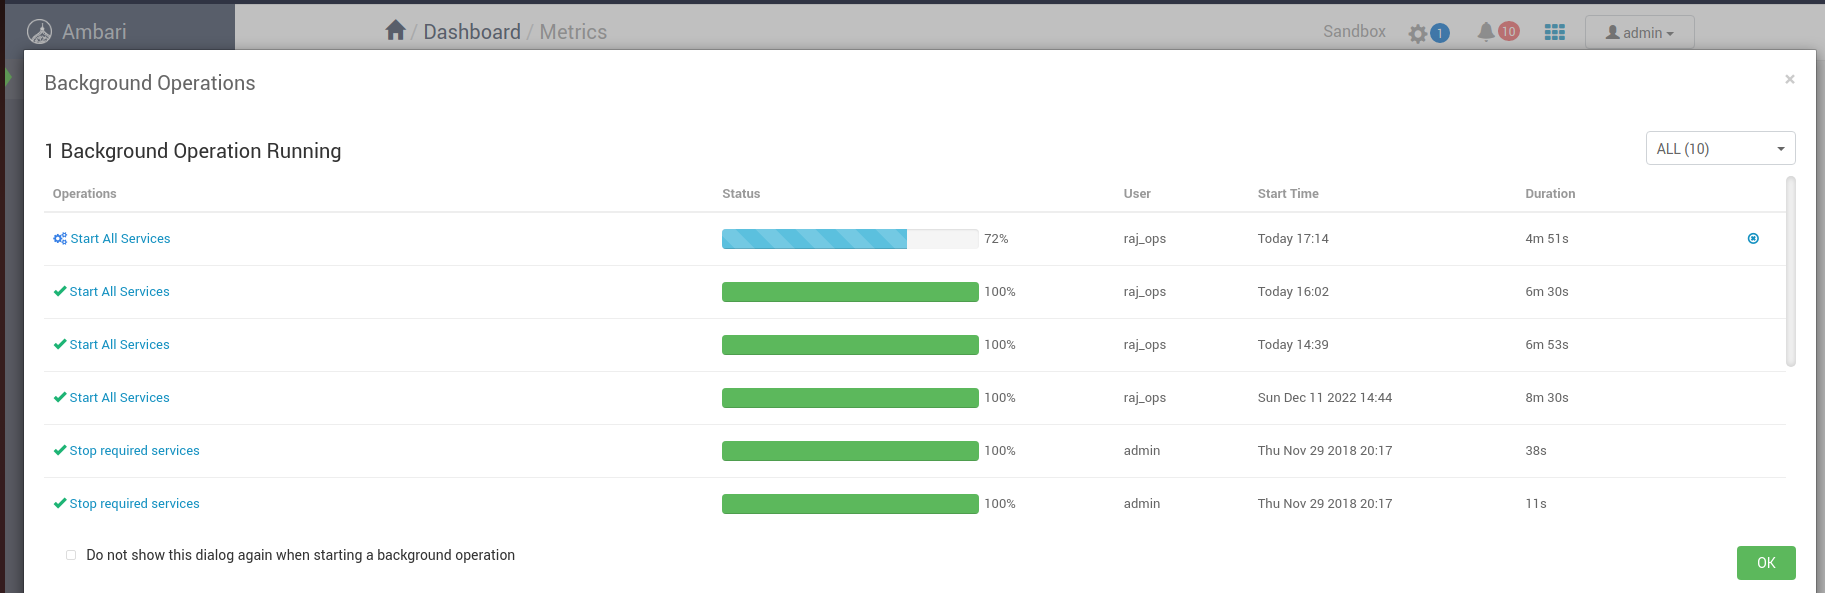
\includegraphics[width=\textwidth]{cluster_startup}
    \caption[Start aller Prozesse beim Cluster Startup]{Start aller Dienste beim Cluster Startup}
    \label{fig:cluster startup}
\end{figure}

Ist der Prozess abgeschlossen, kann man im Navigationsmenü auf der linken Seite unter dem Eintrag \textit{Hosts} eine Auflistung aller Nodes im Cluster (hier nur ein einziger) sehen. Durch Anklicken des Hostnamens gelangt man in die Host-Übersicht, wo man unter anderem die Liste der laufenden Komponenten findet. Abbildung \ref{fig:hdp core processes} zeigt ein Bild davon. Der Übersicht halber wurden nur die Hadoop Core Komponenten abgebildet. Wie man sehen kann, laufen auf diesem Host alle Master-, Worker-, und Client-Prozesse gleichzeitig. Man findet die in Abschnitt \ref{chap:fund sec:core sub:yarn} angesprochenen YARN-Komponenten ResourceManager und NodeManager, die HDFS-Komponenten DataNode und NameNode aus Abschnitt \ref{chap:fund sec:core sub:hdfs}, sowie die Client-Dienste für YARN, HDFS und MapReduce wieder. 

\begin{figure}[ht]
    \centering
    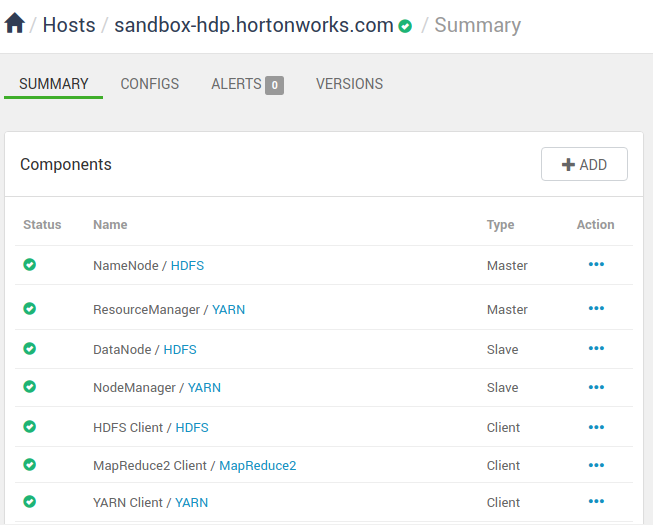
\includegraphics[width= 0.6\textwidth]{hdp_core_processes}
    \caption[Hadoop Core Prozesse in der HDP Sandbox]{Hadoop Core Prozesse in der HDP Sandbox}
    \label{fig:hdp core processes}
\end{figure}

Im Tab \textit{Configs} kann man die sonst über viele XML-Dateien verstreuten Einstellungen der Komponenten vornehmen. So kann man zum Beispiel unter \textit{HDFS -> Advanced -> General -> Block replication} (siehe Abb. \ref{fig:block replication factor}) den Replication Factor des HDFS verändern. Dieser ist in der Sandbox auf \verb|1| gestellt, da es im Single Node Modus nur einen Node gibt und das Speichern mehrerer Block-Replika auf dem gleichen Node keinen Vorteil bringt.  

\begin{figure}[ht]
    \centering
    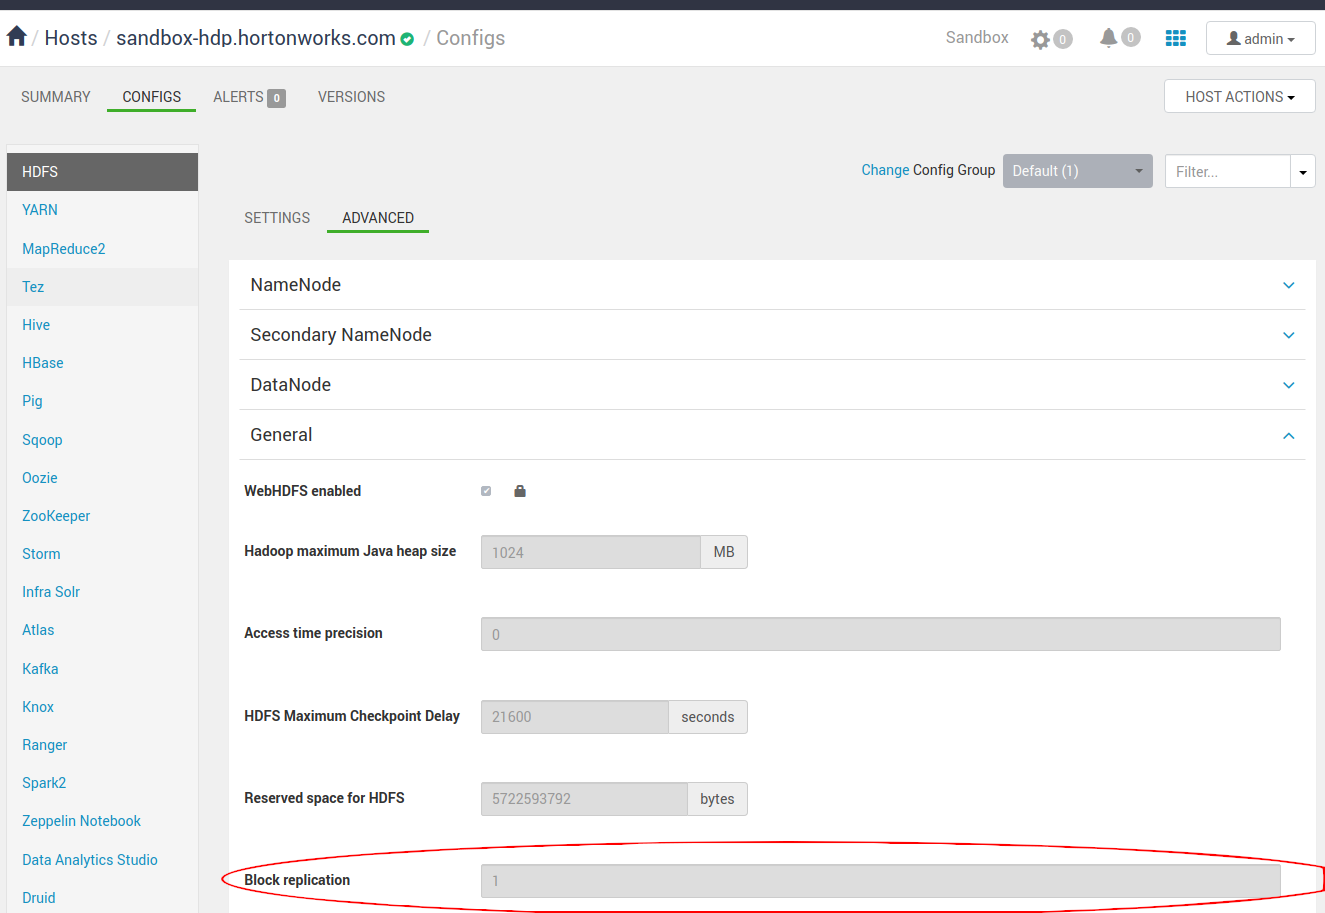
\includegraphics[width=0.85\textwidth]{block_repl_factor}
    \caption[Replication Factor Einstellung in Ambari]{Replication Factor Einstellung in Ambari}
    \label{fig:block replication factor}
\end{figure}


\section{Fallstudie Globales Wetter}
Als Fallstudie für die Nutzung von Hadoop werden die täglichen Zusammenfassungen aller Wetterstationen der Welt aus dem Katalog der National Centers for Environmental Information\footnote{https://www.ncei.noaa.gov/access/search/data-search/global-summary-of-the-day} benutzt. Dieses Beispiel wurde größtenteils entnommen aus \citefield[\textit{(S. 19-30, 693-695)}]{white_hadoop_2015}{title}. Da durch das lokale Setup die Kapazitäten von Hadoop auf die des Host-Computers beschränkt sind, werden hier nur die Datensätze der Jahre 2016 bis 2022 in komprimierten Archiven heruntergeladen\footnote{Download: https://www.ncei.noaa.gov/data/global-summary-of-the-day/archive/}. Diese enthalten jeweils die gesammelten Aufzeichnungen eines Jahres in Form von CSV-Dateien mit geringer Dateigröße (siehe Abb. \ref{fig:ncdc files local}). Das HDFS zeigt jedoch seine Stärken erst bei Datensätzen im Gigabyte- bis Terabyte-Bereich und kann nicht effizient mit vielen kleinen Dateien umgehen\footcite[vgl.][Assumptions and Goals -> Large Data Sets]{noauthor_apache_nodate-1}. 

\begin{figure}[ht]
    \centering
    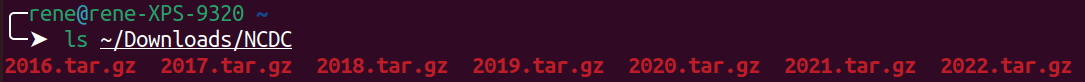
\includegraphics[width=0.7\textwidth]{ncdc_files}
    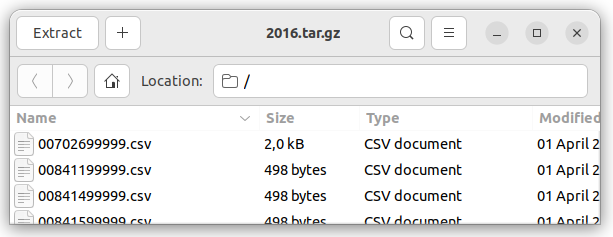
\includegraphics[width=0.7\textwidth]{ncdc_archive_content}
    \caption[NCDC Archive für die Fallstudie]{NCDC Archive für die Fallstudie}
    \label{fig:ncdc files local}
\end{figure}

Das HDFS und MapReduce arbeiten außerdem mit wenigen großen Dateien wesentlich besser als mit vielen kleinen Dateien.\cite[\textit{(S. 19-30, 693-695)}]{white_hadoop_2015} Deshalb wird der erste Schritt sein, die Daten in das HDFS zu laden. Anschließend wird eine MapReduce-Applikation mit der MapReduce Streaming-API geschrieben. Diese wird nur aus einer Map-Phase bestehen und die Dateien säubern und zusammenzuführen. Zuguterletzt wird eine weitere MapReduce-Applikation mit der Java-API geschrieben, die die Daten auswertet. In späteren Abschnitten werden weitere Komponenten des Hadoop Ecosystems vorgestellt, mit denen die Dateien weiter verarbeitet werden.

\section{Umgang mit dem HDFS}
\label{chap:fund sec:core sub:handson hdfs}
Es gibt verschiedene Wege, um Dateien ins HDFS zu laden\footnote{3 Beispiele: https://community.cloudera.com/t5/Support-Questions/Import-data-from-remote-server-to-HDFS/m-p/233149/highlight/true\#M194979}. In der Sandbox wurde ein Ambari View, der \textbf{Files View}\footnote{https://docs.cloudera.com/HDPDocuments/Ambari-2.7.4.0/using-ambari-views/content/\\amb\_using\_files\_view.html}, erstellt. Diesen erreicht man über das Kachel-Icon im Header des Dashboards\footnote{http://<localhost oder Sandbox Hostname>:8080/\#/main/view/FILES/auto\_files\_instance}. Der Files View bietet einen HDFS Dateibrowser mit Funktionalitäten wie Datei-Upload direkt von der lokalen Maschine, Ordnererstellung und Rechteverwaltung. Nicht alle Nutzer der Sandbox haben die nötigen Rechte zur Ausführung der Befehle. Daher sollte man sich mit dem dafür vorgesehenen Nutzer\footnote{https://www.cloudera.com/tutorials/learning-the-ropes-of-the-hdp-sandbox.html\#login-credentials} \verb|user: maria_dev| \verb|password: maria_dev| in Ambari einloggen. Man kann über den Files View aber nur eine Datei zur Zeit hochladen. Das Hochladen von Archiven (gestestet mit \verb|.tar.gz| und \verb|.jar|) schließt ebenfalls nie ab. Da für den nachfolgenden Schritt ein JAR aus dem HDFS als Input eingebunden werden soll, wird ein HDFS Client Prozess verwendet, der mit dem Hadoop Cluster verbunden ist. Dafür ist es nötig, Hadoop lokal installiert zu haben, oder man kopiert erst per \verb|scp| die Dateien auf das lokale Dateisystem eines Nodes im Cluster, auf dem ein HDFS Client läuft. Hierfür verwendet man zum Beispiel den NameNode. 
\par
\textbf{Schritt 1} ist das Erstellen des JARs \verb|ncdc.jar| mit den Eingabedateien des NCDC (siehe Abb. \ref{fig:ncdc jar local}). Hadoop wird dieses nachher dem MapReduce Job bereitstellen und automatisch entpacken. \textbf{Schritt 2} ist das Erstellen der Textdatei \verb|file_names.txt| mit den Dateipfaden der Unterordner des JARs (siehe Abb. \ref{fig:file names txt local}). Diese Datei wird der Input des MapReduce Jobs. 

\begin{figure}[ht]
    \centering
    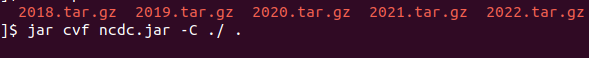
\includegraphics[width=0.75\textwidth]{ncdc_jar_local}
    \caption[Erstellung des JARs mit Wetterdaten]{Erstellung des JARs mit Wetterdaten}
    \label{fig:ncdc jar local}
    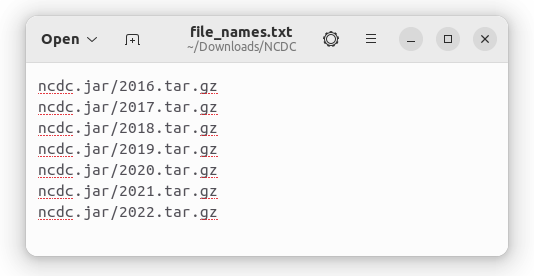
\includegraphics[width=0.75\textwidth]{file_name_list}
    \caption[Inputdatei des MapReduce Jobs]{Inputdatei des MapReduce Jobs}
    \label{fig:file names txt local}
\end{figure}

In \textbf{Schritt 3} gilt es, die bisher erstellten Dateien ins HDFS zu übertragen. Dazu muss man sich per \verb|ssh| als Benutzer \verb|maria_dev| mit der Sandbox verbinden. Um die Ordnerstruktur im HDFS zu erstellen, nutzt man entweder den Ambari File View, oder den Befehl \verb|hdfs dfs -mkdir -p| \verb|/user/maria_dev/input|. \verb|hdfs| ist das Programm zur Interaktion mit dem Hadoop Distributed File System. \verb|dfs| startet die \textbf{Filesystem Shell}, mit der man eine Reihe von ''shell-artigen'' Kommandos\footnote{https://hadoop.apache.org/docs/stable/hadoop-project-dist/hadoop-common/FileSystemShell.html} direkt auf dem HDFS anwenden kann. An dieser Stelle könnte zum Beispiel auch \verb|dfsadmin| stehen, wenn es um die Administration des Dateisystems als solches ginge (einen DataNode abschalten etc.). FS Shell Commands beginnen mit einem Bindestrich, darauf folgt ein Befehl und dahinter kommen die Parameter. \verb|-mkdir -p /user/maria_dev/input| funktoniert genau wie sein Gegenstück aus einer normalen Shell. Der Ordner \verb|input| sollte noch für alle Benutzer als schreibbar markiert werden, da dort hin später die zusammengefassten CSV-Dateien geschrieben werden sollen. Dazu dient der Befehl \verb|hdfs dfs -chmod 777 /user/maria_dev/input|. Ist die Ordnerstruktur erstellt, kann man von seiner lokalen Maschine mit \verb|scp -P <Port> <lokaler Pfad>| \verb|maria_dev@<Hostname>:<Host Pfad>| die bisher erstellten Dateien (JAR und Textdatei) auf das lokale Dateisystem des NameNodes (der Sandbox) kopieren(Abb. \ref{fig:scp transfer}). Anschließend werden diese per FS Shell mit dem Befehl \verb|-moveFromLocal| in das HDFS geladen, damit die Dateien vom lokalen Dateisystem des NameNodes entfernt werden, nachdem sie im HDFS gespeichert wurden (Abb. \ref{fig:hdfs move}).

\begin{figure}[ht]
    \centering
    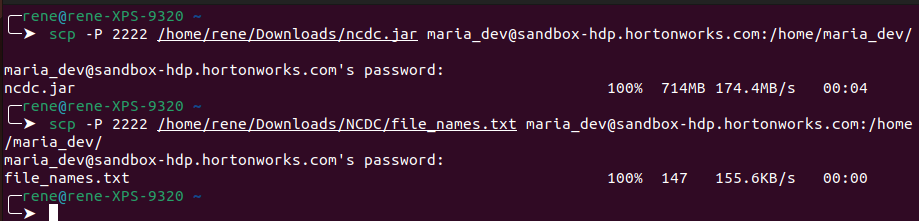
\includegraphics[width=0.75\textwidth]{scp_ncdc_transfer}
    \caption[Dateitransfer mit scp]{Dateitransfer mit scp}
    \label{fig:scp transfer}
    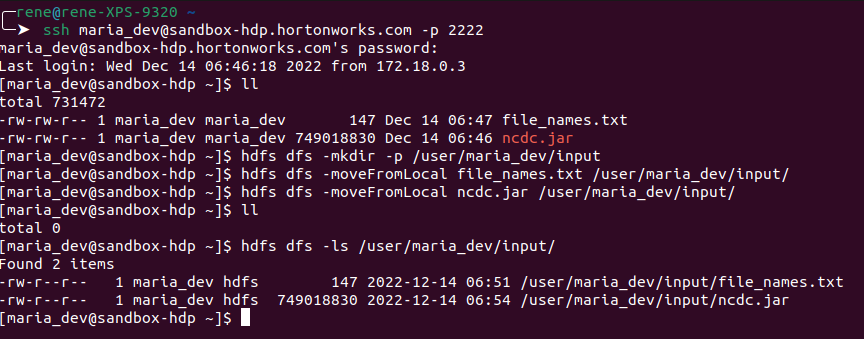
\includegraphics[width=0.75\textwidth]{hdfs_ncdc_move}
    \caption[Dateiupload in das HDFS]{Dateiupload in das HDFS}
    \label{fig:hdfs move}
\end{figure}

\textbf{Schritt 4} ist das Schreiben eines Bash Skripts, welches später als Mapper-Klasse fungiert. Zum Zusammenführen der Dateien wird nicht die Java API von MapReduce, sondern die Streaming API von Hadoop\footnote{https://hadoop.apache.org/docs/stable/hadoop-streaming/HadoopStreaming.html} verwendet. Diese erlaubt es, völlig sprachenunabhängig MapReduce Jobs zu schreiben. Man kann als Mapper und/oder Reducer dabei jeweils eigene Skripte oder Binaries verwenden. Jeder Mapper-Prozess führt eine Instanz des angegebenen Mapper-Skripts aus und füttert ihm, sofern nicht ein anderes InputFormat bestimmt wurde, Zeile für Zeile den Inhalt des ihm zugeteilten InputSplits als Key-Value-Paare auf \verb|stdin|. \verb|stdout| des Skripts wird wiederum vom Mapper zeilenweise als Key-Value-Paar gesammelt und an die Reducer weitergeleitet, wo der Prozess genauso abläuft. Das Skript ist in Listing \ref{lst:ncdc concatenate script} bis auf einige Kommentare abgebildet. Das gesamte Skript findet sich im Appendix \ref{appendix lst:ncdc concatenate script}.    

\lstinputlisting[language=bash, caption={Bash Skript als Mapper-Klasse}, linerange={28-51}, label={lst:ncdc concatenate script}]{code/concatenate_ncdc_data.sh}

Mit \verb|read offset inputfile| liest das Skript das Key-Value-Paar von \verb|stdin| ein. Durch das später bei der Ausführung angegebene InputFormat \verb|NLineInputFormat| ist das erste Wort der Zeile der Offset der Zeile zum Dateianfang. Diese Information ist für diesen Job nicht relevant. Im Rest der Zeile steht der Inhalt der ürsprünglichen Zeile, in diesem Fall ein Dateiname wie \verb|ncdc.jar/20xx.tar.gz|. 
Das Archiv aus dem \verb|ncdc.jar| wird in einen Unterordner in der Laufzeitumgebung des MapReduce Jobs entpackt. Anschließend werden alle darin befindlichen CSV-Dateien zu einer Datei vereint. Diese resultierende Datei wird zum Schluss wieder komprimiert und mit dem Befehl \verb|hdfs dfs -put - <Pfad>| im HDFS abgespeichert. 
\par
\textbf{Schritt 5}:Ist das Skript geschrieben, könnte es wieder per \verb|scp| und \verb|hdfs dfs| in das HDFS übertragen werden. An dieser Stelle soll aber der Ambari File View gezeigt werden. Zu diesem navigiert man wie bereits in Abschnitt \ref{chap:fund sec:core sub:handson hdfs} beschrieben und wechselt über die grafische Oberfläche in den Zielordner \verb|/user/maria_dev/input|. Über den Upload Button oben rechts kann man die Datei direkt von seinem lokalen Rechner ins HDFS laden. Am Ende sollte der Inhalt des Ordners aussehen wie in Abbildung \ref{fig:ncdc files hdfs}. Das Skript muss noch für alle Nutzer als ausführbar markiert werden, damit der MapReduce Job es später benutzen kann. Dafür wählt man die Datei an, klickt oben links auf \verb|Permissions| und setzt sie entsprechend Abbildung \ref{fig:concat script permissions}. Man könnte hierfür auch das HDFS CLI mit dem Befehl \verb|hdfs dfs -chmod 755 <Pfad>| verwenden.

\begin{figure}[ht]
    \centering
    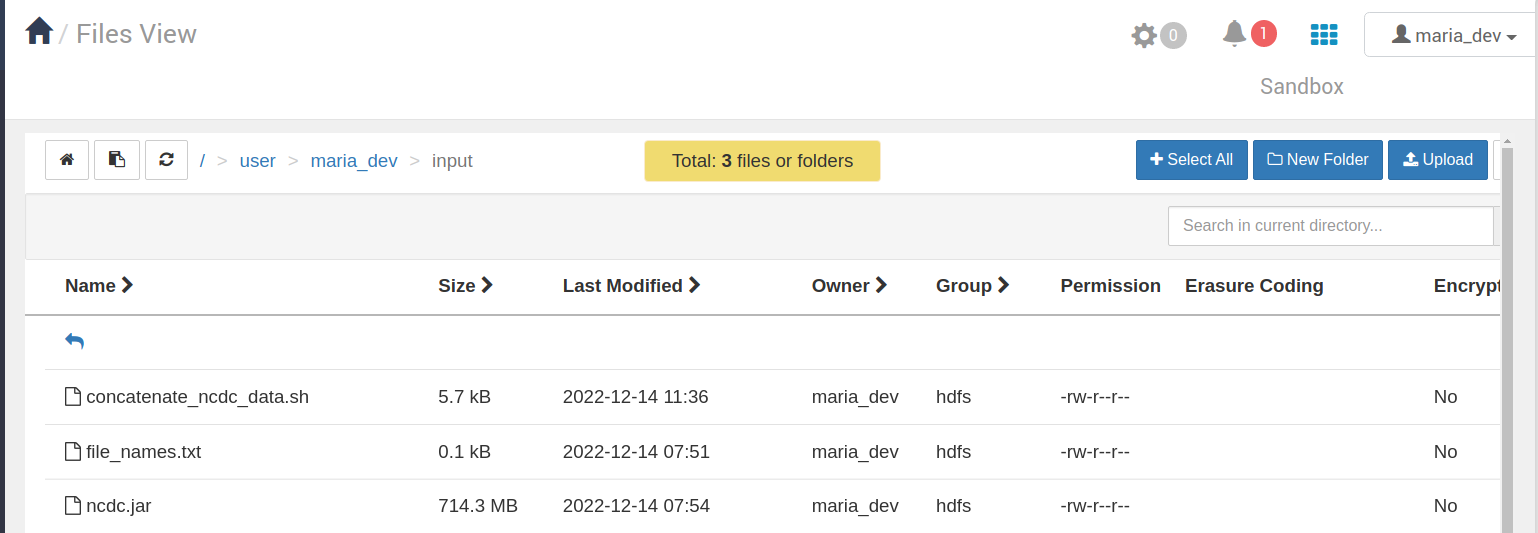
\includegraphics[width=0.9\textwidth]{ncdc_files_on_hdfs}
    \caption[Upload der NCDC Datensätze]{Upload der NCDC Datensätze}
    \label{fig:ncdc files hdfs}
    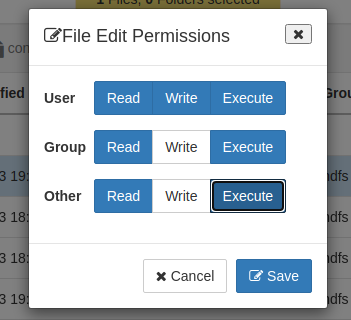
\includegraphics[width=0.5\textwidth]{script_permissions}
    \caption[Setzen von Dateiberechtigungen im Ambari File View]{Setzen von Dateiberechtigungen im Ambari File View}
    \label{fig:concat script permissions}
\end{figure}


\section{MapReduce mit der Hadoop Streaming API}
\label{chap:fund sec:core sub:handson mapred streaming}
Um den vorbereiteten MapReduce Job auszuführen, muss der Befehl aus Listing \ref{lst:ncdc concatenate start script} abgesetzt werden. Der vollständig dokumentierte Befehl ist in Appendix \ref{appendix lst:ncdc concatenate start script} zu finden. 

\begin{itemize}
    \item Zeile 1 weist Hadoop an, ein JAR auszuführen. Dateipfad des Hadoop Streaming JARs angegeben, welches mit dem Framework mitgeliefert wird.
    \item Zeile 2 sorgt dafür, dass Hadoop das im HDFS gespeicherte JAR \verb|ncdc.jar| in die Laufzeitumgebung des MapReduce Jobs kopiert und automatisch entpackt. Prozesse können während des Jobs unter dem Pfad \verb|ncdc.jar| auf die darin enthaltenen Dateien (hier die TARs mit den jährlichen Datensätzen) zugreifen.
    \item Zeile 3 weist Hadoop eigentlich an, die Mapper-Klasse vom lokalen Dateisystem auf alle am Job beteiligten Nodes zu kopieren, damit sie dort lokal zur Verfügung steht. Durch das Präfix \verb|hdfs://host:port/| teilt man Hadoop mit, dass die Datei bereits im HDFS liegt. Mit \verb|\#concatenate\_ncdc\_data.sh| am Ende des Pfades gibt man der Datei einen Alias, damit man in der \verb|-mapper| Option nicht wieder den vollen Pfad angeben muss.      
    \item Mit \verb|-D| kriegt ein Parameter Priorität über eine Einstellung, die bereits in Konfigurationsdateien gesetzt sind.
    \item Zeile 4 macht aus diesem Job einen reinen Map-Job ohne Reduce-Phase, da für die Umwandlung der Dateien keine Reduce-Phase nötig ist.
    \item Zeile 5 verhindert die sogenannte spekulative Ausführung. Ist diese Option aktiviert, startet Hadoop manchmal mehrere Jobs für einen InputSplit und filtert in der Shuffle-Phase doppelte Ergebnisse. Sind manche Nodes deutlich langsamer als andere, kann das Performancegewinne bringen. In diesem Fall würde das aber dazu führen, dass Dateien doppelt ins HDFS geschrieben würden, da nicht der Output der Mapper verwendet wird, sondern das Skript direkt ins HDFS schreibt.
    \item Zeile 6 gibt den Pfad zur Datei im HDFS an. Anders als bei der Angabe des mitzuliefernden JARs muss bei den Parametern für Input und Output kein vollständiger HDFS-Pfad angegeben werden. MapReduce erwartet standardmäßig, dass es sich dabei um Verzeichnisse und Dateien im HDFS handelt.
    \item Zeile 7 gibt die Java Klasse des InputFormats an. Diese gehört zum Hadoop Framework und ist im Java Class Path der Ausführungsumgebung verfügbar. Mit \verb|NLineIn-| \verb|putFormat| werden einem Mapper \textit{N} Zeilen aus dem InputSplit als Eingabe gegeben. \textit{N} ist standardmäßig \verb|1|. 
    \item Zeile 8 gibt den Pfad an, unter dem die Reducer ihre Ausgabedateien ablegen werden. Es muss sich hierbei um einen Ordner handeln, der noch nicht existiert. Im HDFS können Dateien nicht einfach überschrieben werden. Daher dürfen Ausgabeordner grundsätzlich nicht vorher existieren.
    \item Zeile 9 gibt die Mapper-Klasse an. Würde die Java API statt der Streaming API verwendet, stünde hier eine Java Klasse. Es wird der Alias aus Zeile 3 benutzt.
\end{itemize}

\lstinputlisting[language=bash, linerange={7-15}, caption={Startskript für den NCDC Concatenation MapReduce Job}, label={lst:ncdc concatenate start script}]{code/concat_files_start.sh}

Sind alle Dateien an den richtigen Orten platziert, kann man sich erneut als \verb|maria_dev| per \verb|ssh| auf den NameNode verbinden und den Befehl aus Listing \ref{lst:ncdc concatenate start script} absetzen. Die Ausführung kann mehrere Minuten dauern. Am Ende sollte die Konsole eine ähnliche Ausgabe wie in Abbildung \ref{fig:ncdc concat console output} zeigen. Es wurden der Übersicht halber viele Zeilen in der Abbildung entfernt. Man kann sehen, dass der Job ein Input File (die \verb|file_names.txt|) gelesen und daraus sieben InputSplits erstellt hat, korrespondierend zu den sieben Zeilen (Dateipfaden) in der Datei. Für jeden InputSplit wurde ein Mapper gestartet und alle Mapper sind haben ihre Arbeit erfolgreich beendet. Mit der \verb|applicationId| \verb|application_xxxxxxxxxxx_xxxx| kann man die YARN Logs zum Job Run anzeigen lassen. Darin findet man unter anderem die Statusreports aus dem Skript und eventuelle Fehlermeldungen. Dieser MapReduce Job schließt nämlich auch erfolgreich ab, wenn beim Entpacken oder Zusammenfügen der Archive ein Fehler auftritt, da diese Vorgänge als Unterprozesse des eigentlichen Mappers ohne Fehlerüberprüfung ausgeführt wurden. Sind zum Beispiel die Rechte auf dem Ordner, in den die fertigen Dateien mit \verb|hdfs dfs -put -| geschrieben werden sollen, falsch gesetzt, wird man dies nur anhand der fehlenden Dateien und der YARN Logs bemerken. Existiert jedoch der Ordner bereits, der als Ausgabeverzeichnis des Jobs angegeben wurde, oder kann eine die Eingabedatei nicht gefunden werden, beendet sich der MapReduce Job mit einer entsprechenden Fehlermeldung. Weiter unten in der Konsolenausgabe sieht man, dass die Mapper insgesamt über elf Minuten Laufzeit benötigt haben. Den Zeitstempeln kann man aber entnehmen, dass der Job nur etwas über vier Minuten lief. Daran sieht man den Performancegewinn bei paralleler Verarbeitung der Daten. Im Single Node Setup ist zwar nur ein Node an der Verarbeitung beteiligt, aber Hadoop startet mehrere JVM-Prozesse, welche dann auf mehreren Prozessorkernen gleichzeitig laufen können.

\begin{figure}[ht]
    \centering
    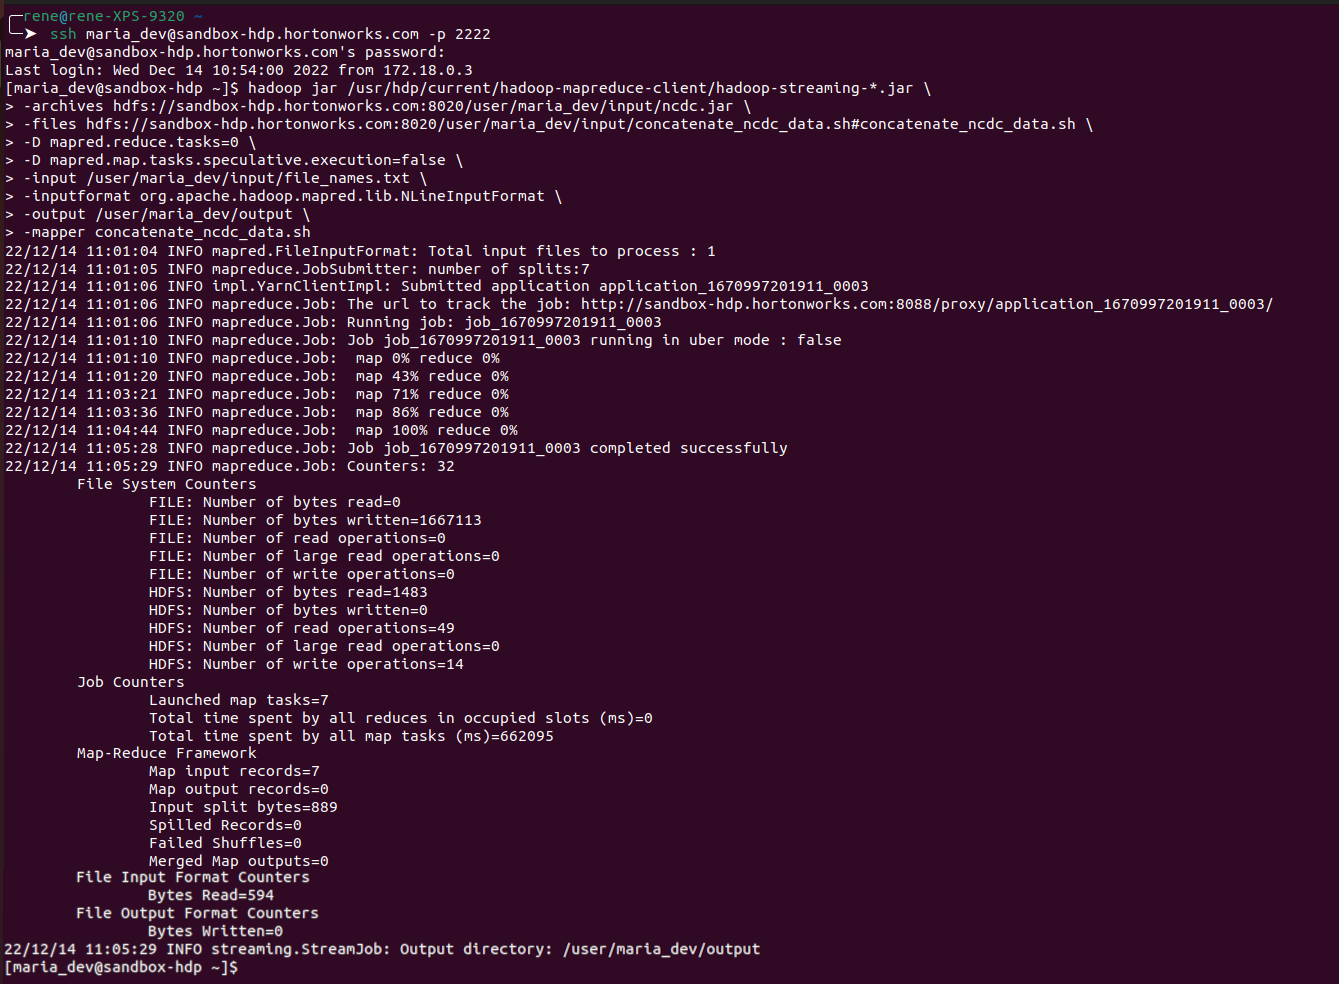
\includegraphics[width=\textwidth]{ncdc_concat_console_output}
    \caption[MapReduce Konsolenausgabe]{MapReduce Konsolenausgabe}
    \label{fig:ncdc concat console output}
\end{figure}

Die Ausgabedateien des Jobs können ebenfalls betrachtet werden. Ein Blick in den File View zeigt, dass Hadoop den Ordner \verb|/user/maria_dev/output|, wie im \verb|-output|-Parameter gefordert, angelegt hat. In diesem Ordner befinden sich sieben Dateien mit den Namen \verb|part-0000x| (siehe Abb. \ref{fig:ncdc concat mr output}). Diese Dateien sind die Ausgaben der Mapper. Da der Job keine Reducer verwendet hatte, wurde eine Datei pro Mapper erstellt. Da die Mapper aber keine Ausgaben erzeugt haben, was bei der Streaming API durch Schreiben auf \verb|stdout| passiert wäre, sind diese Dateien vollkommen leer. Eine achte Datei im Ordner gibt mit ihrem Namen den Exit-Status des Jobs an, hier \verb|_SUCCESS|.

\begin{figure}[ht]
    \centering
    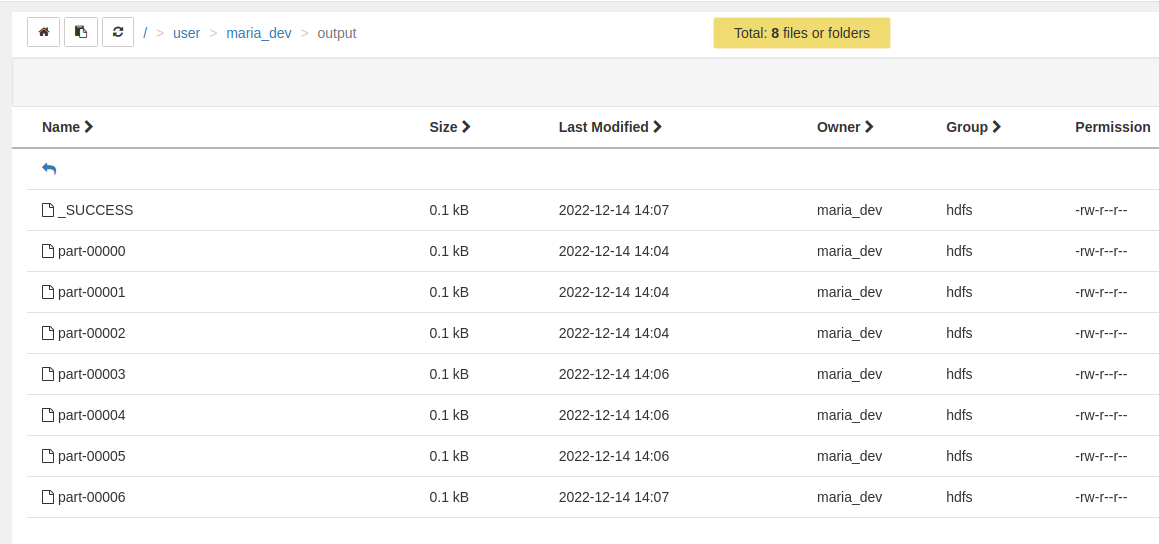
\includegraphics[width=0.8\textwidth]{ncdc_concat_mr_output_files}
    \caption[MapReduce Ausgabedateien]{MapReduce Ausgabedateien}
    \label{fig:ncdc concat mr output}
\end{figure}

Im Ordner \verb|/user/maria_dev/input/processed| liegen die zusammengefassten und erneut komprimierten Dateien ab, die während der Map-Phase des Jobs erstellt wurden (siehe Abb. \ref{fig:ncdc concat final output}). Diese kann man im Webbrowser über den \textit{Open} Button direkt betrachten. Die Anzeige funktioniert nicht fehlerfrei; es sind abgehackte und duplizierte Zeilen zu sehen (siehe Abb. \ref{fig:buggy web output}). Dies sind allerdings nur Fehler des File Views. Lädt man die Dateien wieder herunter und betrachtet sie lokal, wird man feststellen, dass das Zusammenfügen funktioniert hat. Lediglich die Headerzeile wiederholt sich mehrmals in jeder Datei, was im weiteren Verlauf der Bearbeitung beachtet werden muss.

\begin{figure}[ht]
    \centering
    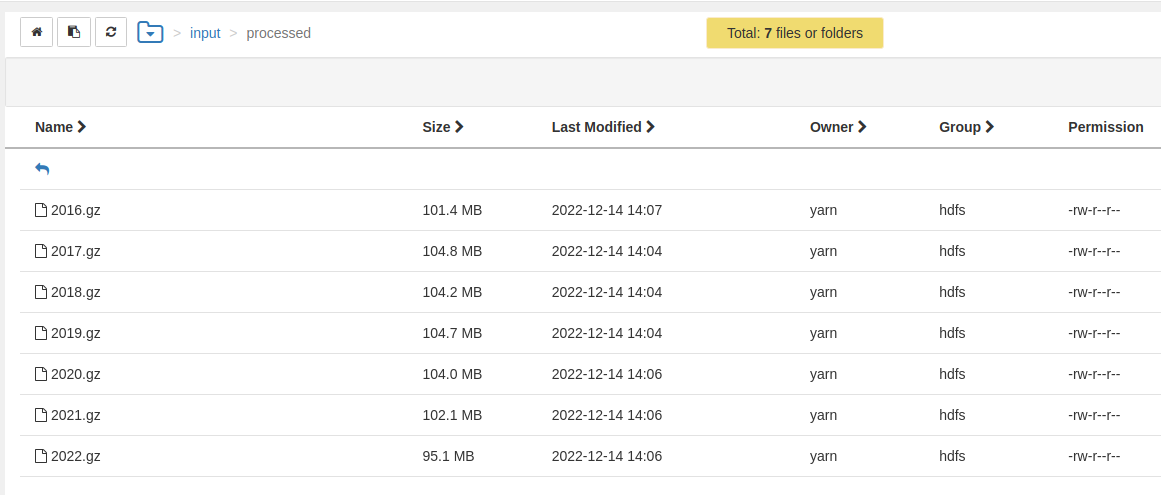
\includegraphics[width=0.8\textwidth]{ncdc_concat_combined_output_files}
    \caption[Zusammengefügte, komprimierte Wetterdaten im HDFS]{Zusammengefügte, komprimierte Wetterdaten im HDFS}
    \label{fig:ncdc concat final output}
    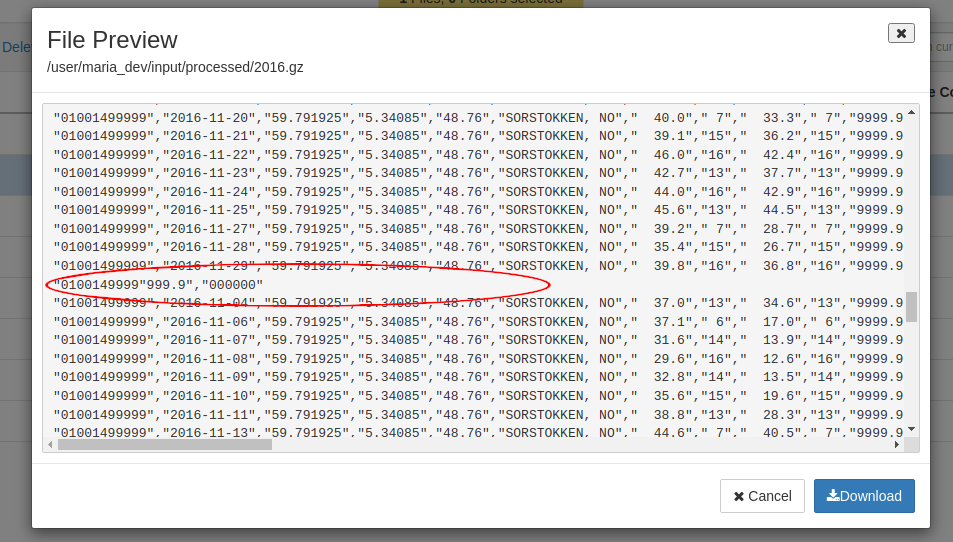
\includegraphics[width=0.8\textwidth]{buggy_web_view}
    \caption[Fehlerhafte Anzeige der Daten im File View]{Fehlerhafte Anzeige der Daten im File View}
    \label{fig:buggy web output}
\end{figure}

\section{Die MapReduce Java API}
\label{chap:fund sec:core sub:handson mapred java}




